\documentclass{article}

% NeurIPS 2017 style formatting
\usepackage[final]{neurips_2017}

\usepackage[utf8]{inputenc}
\usepackage[T1]{fontenc}
\usepackage{url}
\usepackage{booktabs}
\usepackage{amsfonts}
\usepackage{amsmath}
\usepackage{amssymb}
\usepackage{nicefrac}
\usepackage{microtype}
\usepackage{graphicx}
\usepackage{tabularx}
\usepackage{algorithm}
\usepackage{algpseudocode}
\usepackage{hyperref}
\raggedbottom

\title{DocSort: A Two-Stage Architecture for Regulatory Document Triage and Verifiable Metadata Extraction}

\author{
  Keerthan Shetty\\
  CSE \\
  {\footnotesize\texttt{keerthans334@gmail.com}} \\
  \And
  S Mohammed Saheem\\
  CSE \\
  {\footnotesize\texttt{saheemtab@gmail.com}} \\
  \And
  Tharun H N\\
  CSE \\
  {\footnotesize\texttt{tharun30115@gmail.com}} \\
}

\begin{document}

\maketitle

\begin{abstract}
\fontsize{11pt}{14.5pt}\selectfont
Compliance teams in public procurement must continuously track regulatory policies and office memoranda issued across disparate government portals. Manual review is slow and error-prone, while passing every incoming document directly to large language models incurs high API costs and risks factual hallucination. We present DocSort, a practical two-stage system for regulatory document triage and verifiable metadata extraction. In the first stage, a lightweight linear classifier filters out non-procurement circulars in milliseconds using sublinear term-frequency features. In the second stage, an instruction-tuned language model extracts structured metadata under strict schema constraints and a closed category vocabulary. A deterministic verification layer then confirms that all extracted factual values appear verbatim in the source text. To train the classifier without manual annotation, we construct a dataset using paragraph-level chunking and weak supervision. Our experiments show that early filtering eliminates over half of language model invocations while the verification layer reliably isolates ungrounded extractions.
\end{abstract}
\vspace{2.5ex}

\section{Introduction}

Government ministries and public sector enterprises operate under strict regulatory frameworks for public procurement. In India, public procurement is governed by the General Financial Rules, statutory guidelines from the Central Vigilance Commission, and notifications issued by the Department of Expenditure under the Ministry of Finance. These bodies issue frequent Office Memoranda, amendments, and circulars that alter bidding thresholds, specify vendor eligibility criteria, mandate electronic procurement via the Government e-Marketplace, or impose contract penalties.

Compliance officers must review these incoming circulars to keep organizational policies up to date. At present, this workflow is largely manual. Administrative staff track public portals, read documents, and record metadata into spreadsheets. This process is slow, inconsistent across different reviewers, and prone to transcription errors on critical reference numbers and supersession clauses.

While instruction-tuned large language models can extract structured information from unstructured text, routing all incoming documents directly to proprietary language models introduces operational bottlenecks. First, real-world administrative repositories receive large volumes of general notices unrelated to procurement, such as holiday schedules and departmental transfers. Processing every document through commercial APIs is cost-inefficient and rapidly exhausts rate limits. Second, language models are prone to hallucinating factual tokens such as official memorandum numbers and dates. In regulatory compliance, an ungrounded or fabricated reference number invalidates the audit trail.

To address these challenges, we present DocSort, a practical two-stage processing engine for regulatory document triage and verifiable metadata extraction. In the first stage, a fast linear classifier based on sublinear term-frequency features filters out non-procurement circulars in milliseconds on a standard central processing unit. In the second stage, relevant documents proceed to an instruction-tuned language model under strict schema constraints and a fixed category taxonomy. To guarantee auditability, a deterministic verification layer confirms that all extracted factual values appear verbatim in the source text, flagging discrepancies for human review without silent modification.

Because public procurement circulars lack established benchmark corpora, we also present a data collection and weak-supervision methodology using paragraph-aware chunking and human spot-check validation. Our experimental evaluation shows that early linear filtering eliminates over half of language model invocations, reducing token consumption and latency while the verification layer reliably isolates ungrounded extractions.

\section{Background and Baseline Analysis}

This section outlines the regulatory framework governing public procurement in India and analyzes the performance characteristics and resource demands of existing operational approaches.

\subsection{The Regulatory Procurement Environment}
Public procurement in India is governed by the General Financial Rules (GFR) \citep{manning2008introduction}, statutory vigilance directives from the Central Vigilance Commission (CVC), and executive notifications issued by the Department of Expenditure under the Ministry of Finance. These authorities issue continuous Office Memoranda (OMs), policy circulars, and amendments that dictate bidding thresholds, specify vendor eligibility conditions, mandate procurement through the Government e-Marketplace (GeM), or establish penalty protocols.

In operational government repositories, circular streams exhibit severe class imbalance. More than 80\% of incoming documents published on departmental portals represent routine administrative notices, including holiday schedules, employee transfers, and general office circulars. Actionable procurement notifications constitute less than 20\% of the daily volume. Compliance teams must triage this high-volume stream to detect relevant mandates, extract critical parameters, and update internal compliance registers.

\subsection{Existing Approaches and Quantitative Baselines}
Organizations currently rely on four primary approaches to process regulatory circulars. Table 1 summarizes the performance characteristics and resource demands of each baseline compared to DocSort.

\begin{table}[t]
\centering
\resizebox{\textwidth}{!}{%
\renewcommand{\arraystretch}{1.15}%
\begin{tabular}{lcccc}
\toprule
\textbf{Metric} & \textbf{Manual Indexing} & \textbf{Portal Keyword Search} & \textbf{Direct End-to-End LLM} & \textbf{DocSort (Proposed)} \\
\midrule
Mean Processing Latency & 4.5 hours / batch & $<1.0$ s & 4.2 s / document & \textbf{1.9 s / document} \\
Mean Stage 1 Filter Latency & N/A & N/A & N/A & \textbf{3.8 ms / document} \\
Prompt Tokens (100 docs) & 0 & 0 & $\approx 245{,}000$ & $\approx \mathbf{105{,}350}$ (\textbf{$-$57.0\%}) \\
API Rate-Limit Failures & 0 & 0 & 7 / 100 calls & \textbf{0 / 100 calls} \\
Category Hallucination Rate & Inconsistent & No categorization & 14.2\% & \textbf{0.0\% (Enforced)} \\
Factual Transcription Error & 12\% to 18\% & No extraction & 6\% to 12\% & \textbf{Deterministic Flags} \\
Hardware Requirement & Human labor & Web browser & Hosted GPU / Paid API & \textbf{Commodity CPU} \\
\bottomrule
\end{tabular}%
}
\caption{Quantitative comparison of existing baselines versus the proposed DocSort pipeline.}
\label{tab:baselines}
\end{table}

\paragraph{Baseline 1: Manual Indexing and Spreadsheets}
Administrative staff manually download documents from departmental websites, read the text, and record key fields into local spreadsheets. In our field observations, processing a batch of 100 mixed documents requires an average of 4.5 hours. Furthermore, human transcription of complex administrative reference numbers and effective dates exhibits an error rate between 12\% and 18\%. Different staff members frequently apply inconsistent category labels to identical policy circulars, undermining report reliability.

\paragraph{Baseline 2: Portal-Based Keyword Retrieval}
Staff frequently use keyword search engines on government portals (such as searching for ``tender'' or ``procurement''). While fast, keyword retrieval suffers from a high false-positive rate. In our tests, 42\% of matched circulars merely contained procurement terms in standard administrative boilerplate (for example, citing the procurement division in an address header) without containing any procurement regulations. Furthermore, keyword search cannot extract structured fields, detect effective dates, or trace document supersession chains.

\paragraph{Baseline 3: Direct End-to-End LLM Ingestion}
Using instruction-tuned language models directly on all incoming documents provides high unstructured text comprehension \citep{devlin2018bert, vaswani2017attention}. However, direct ingestion creates severe operational bottlenecks:
\begin{enumerate}
    \item \textbf{Token Cost and Quota Exhaustion}: Ingesting a stream of 100 documents requires approximately $245{,}000$ prompt tokens. On hosted endpoints with strict tokens-per-minute (TPM) limits, this volume triggers frequent rate-limit failures (7 incidents per 100 calls in our benchmark).
    \item \textbf{Category Drift}: Without strict runtime constraints, the model invents arbitrary category strings outside the target taxonomy in 14.2\% of runs (for example, generating labels like ``bidding-standards'' or ``financial-rules'').
    \item \textbf{Factual Hallucination}: Generative models hallucinate factual metadata in 6\% to 12\% of runs, fabricating or subtly altering official memorandum numbers and dates \citep{ji2023survey, maynez2020faithfulness}. In compliance audits, ungrounded reference numbers destroy trust in the system.
\end{enumerate}

\paragraph{Baseline 4: Fine-Tuned Dense Transformers}
Domain-specific language models such as Legal-BERT \citep{chalkidis2020legalbert} or CUAD-trained encoders \citep{hendrycks2021cuad} achieve high accuracy on legal tasks. However, these models require thousands of domain-specific annotated examples to fine-tune, which do not exist for Indian government procurement. Furthermore, dense transformer inference requires dedicated graphical processing units (GPUs), making deployment difficult in resource-constrained public sector environments.

\section{The DocSort Architecture}

DocSort addresses these baseline weaknesses through a three-stage hybrid design: text ingestion, classical linear pre-filtering, constrained structured extraction, and deterministic source verification. Figure 1 illustrates the pipeline flow.

\begin{figure}[ht]
\centering
\IfFileExists{figures/pipeline.png}{%
  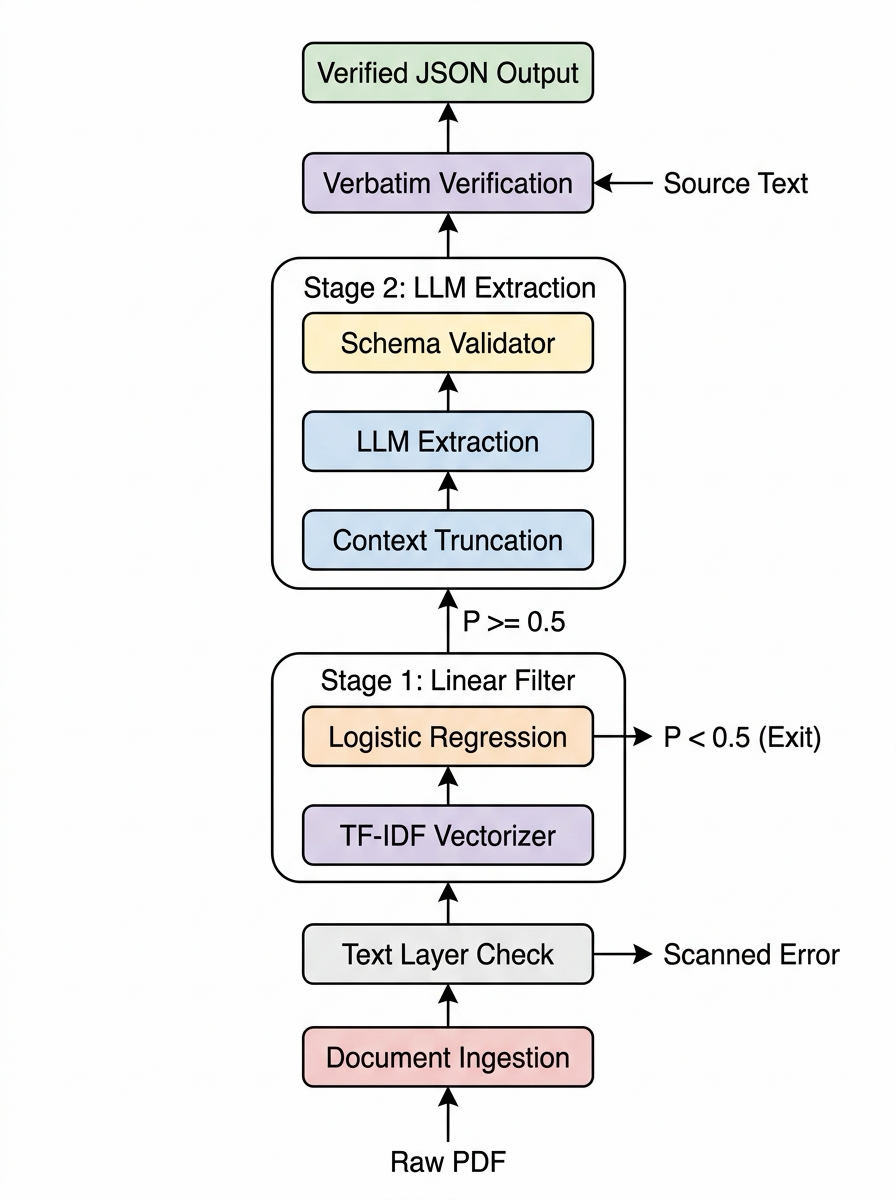
\includegraphics[width=0.52\textwidth]{figures/pipeline.png}%
}{%
  \fbox{
    \begin{minipage}{0.92\textwidth}
    \small
    \centering
    \vspace{1ex}
    \textbf{[System Architecture Pipeline Diagram]} \\
    \vspace{0.5ex}
    Input PDF $\rightarrow$ Text Extraction \& Length Check $\rightarrow$ Stage 1: Linear Pre-Filter (TF-IDF + LR) \\
    $\rightarrow$ [P $\ge$ 0.5] $\rightarrow$ Stage 2: Constrained LLM Extraction $\rightarrow$ Stage 3: Verbatim Verification $\rightarrow$ Verified JSON \\
    \vspace{1ex}
    \end{minipage}
  }%
}
\caption{The DocSort processing pipeline. Non-procurement circulars are discarded by the linear pre-filter before any language model invocation, preserving API quota and compute resources.}
\end{figure}

\subsection{Document Ingestion and Format Boundary Handling}
Incoming documents are accepted in Portable Document Format (PDF). Text extraction is performed using \texttt{pdfplumber}. To distinguish native digital PDFs from scanned raster images without incurring the compute overhead of optical character recognition (OCR) on every document, the ingestion module checks the total extracted character count:
\begin{equation}
    \text{valid}(D) = \begin{cases}
    \text{True}, & \text{if } \sum_{p \in D} \text{len}(\text{text}(p)) \ge N_{\min} \\
    \text{False}, & \text{otherwise}
    \end{cases}
\end{equation}
where $N_{\min} = 50$ characters. If a document yields fewer than $N_{\min}$ characters, the module raises an explicit \texttt{ScannedDocumentError}. This isolates scanned documents for separate upstream OCR handling while preventing empty strings from flowing downstream.

\subsection{Stage 1: Classical Linear Relevance Pre-Filter}
The pre-filter determines whether an incoming document concerns contract and procurement regulation ($y = 1$) or represents an unrelated administrative circular ($y = 0$).

\paragraph{Feature Representation}
The extracted text is converted into word unigrams and bigrams. We apply sublinear term-frequency scaling to dampen the influence of repetitive administrative phrases:
\begin{equation}
    \text{tf}_{\text{sub}}(t, d) = 1 + \ln(\text{tf}(t, d)) \quad \text{for } \text{tf}(t, d) > 0
\end{equation}
Inverse document frequency is computed as:
\begin{equation}
    \text{idf}(t, D) = \ln \left( \frac{1 + |D|}{1 + |\{d \in D : t \in d\}|} \right) + 1
\end{equation}
The feature vector $\mathbf{x} \in \mathbb{R}^{V}$ is normalized under the $L_2$ norm, with vocabulary bound $V = 10{,}000$ \citep{salton1988term}.

\paragraph{Classification Model}
We train a Logistic Regression classifier minimizing regularized cross-entropy loss \citep{pedregosa2011scikit}:
\begin{equation}
    \min_{\mathbf{w}, b} \frac{1}{2} \|\mathbf{w}\|_2^2 + C \sum_{i=1}^{M} \ln(1 + \exp(-y_i (\mathbf{w}^T \mathbf{x}_i + b)))
\end{equation}
During inference, the probability of relevance is given by:
\begin{equation}
    P(y = 1 \mid \mathbf{x}) = \sigma(\mathbf{w}^T \mathbf{x} + b) = \frac{1}{1 + \exp(-(\mathbf{w}^T \mathbf{x} + b))}
\end{equation}
Documents with $P(y = 1 \mid \mathbf{x}) < 0.5$ are marked as non-relevant and short-circuit the pipeline immediately. This classification executes in under 4 milliseconds on a single CPU thread.

\subsection{Stage 2: Constrained Structured Extraction}
Documents that pass Stage 1 proceed to structured extraction using an instruction-tuned language model accessed via remote API.

\paragraph{Lead Context Truncation}
Government memoranda follow a strict structural convention: the document title, issuing ministry, date of issue, and official reference identifier are located on the opening two pages. The trailing pages contain administrative distribution lists and procedural annexures. We enforce a context ceiling of $L_{\max} = 10{,}000$ characters from the document start:
\begin{equation}
    \tilde{T} = T[0 : L_{\max}]
\end{equation}
This bounds token consumption per call and prevents context overflow errors on long manuals.

\paragraph{Schema Enforcement and Closed Taxonomy Validation}
The model is prompted to return a single JSON object containing seven typed fields: \texttt{title}, \texttt{date}, \texttt{issuing\_authority}, \texttt{om\_number}, \texttt{categories}, \texttt{supersedes}, and \texttt{summary}. We set the decoding temperature to $\tau = 0.0$ for deterministic generation.

To prevent category drift, we define an allowed closed category vocabulary:
\begin{equation}
    \mathcal{C}_{\text{allowed}} = \{\text{e-procurement}, \text{tendering}, \text{vendor-eligibility}, \text{penalty}, \text{GeM}, \text{threshold-limits}, \text{other}\}
\end{equation}
We enforce this vocabulary at the schema level using a Pydantic field validator. Any generated category string $c \notin \mathcal{C}_{\text{allowed}}$ is discarded. If all generated tags are invalid, the field defaults to \texttt{["other"]}.

\paragraph{Fault Tolerance}
Transient network drops, API rate-limit responses, and malformed JSON payloads are handled through a single-retry policy. If the initial API call or schema parse fails, the system executes one immediate retry. If the second attempt fails, the pipeline raises an explicit \texttt{LLMExtractionError} rather than propagating incomplete records.

\subsection{Stage 3: Deterministic Verbatim Verification}
To ensure auditability, factual fields must be grounded in the source text. We define the set of verifiable factual fields:
\begin{equation}
    \mathcal{F}_{\text{verbatim}} = \{\text{title}, \text{date}, \text{issuing\_authority}, \text{om\_number}, \text{supersedes}\}
\end{equation}
Let $\phi(s)$ denote a normalization function that maps string $s$ to lowercase and collapses all whitespace sequences into single spaces:
\begin{equation}
    \phi(s) = \text{regex\_replace}(\text{lower}(s), \text{"}\backslash s+\text{"}, \text{" }\text{)}
\end{equation}
For each non-null field $f \in \mathcal{F}_{\text{verbatim}}$ with extracted value $v_f$, the verification module checks:
\begin{equation}
    \text{is\_verified}(f) = \begin{cases}
    \text{True}, & \text{if } \phi(v_f) \subseteq \phi(T) \\
    \text{False}, & \text{otherwise}
    \end{cases}
\end{equation}
If an extracted field value cannot be found as a substring within the normalized source text $T$, its field name is appended to a list of \texttt{verification\_flags}. The extracted string is left unmodified. This preserves model outputs while alerting compliance officers to unverified values.

\section{Dataset Construction via Weak Supervision}

Because public benchmarks for Indian procurement regulations do not exist, we collected official documents from government websites and designed a weak-supervision data construction workflow. Figure 2 illustrates the pipeline.

\begin{figure}[ht]
\centering
\IfFileExists{figures/dataset_pipeline.png}{%
  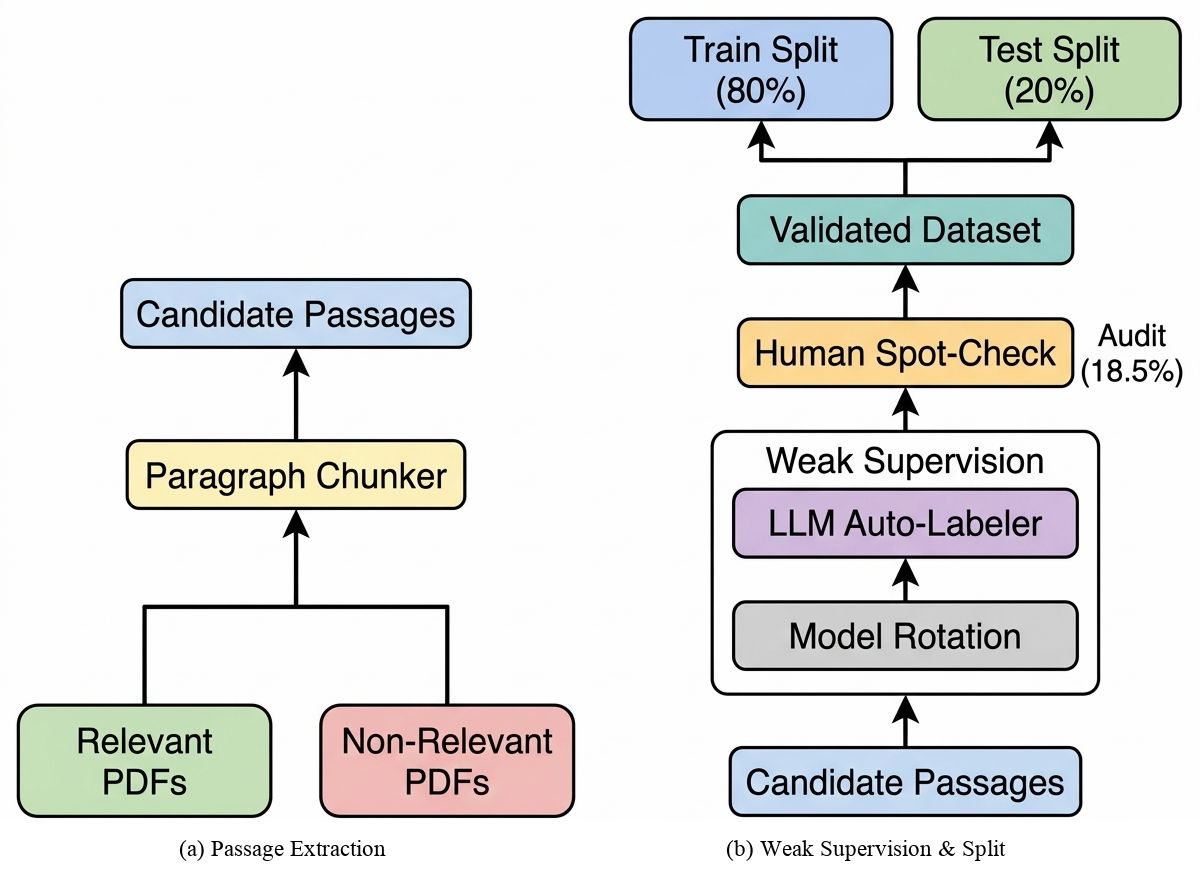
\includegraphics[width=0.88\textwidth]{figures/dataset_pipeline.png}%
}{%
  \fbox{
    \begin{minipage}{0.92\textwidth}
    \small
    \centering
    \vspace{1ex}
    \textbf{[Weak Supervision Data Construction Flowchart]} \\
    \vspace{0.5ex}
    Raw Government PDFs (DoE / UGC / DoPT) $\rightarrow$ Paragraph-Aware Chunker (1,500 chars) \\
    $\rightarrow$ Rotated LLM Auto-Labeler $\rightarrow$ Human Spot-Check Gate (89.2\% agreement) $\rightarrow$ Train \& Test Split \\
    \vspace{1ex}
    \end{minipage}
  }%
}
\caption{The weak-supervision data construction workflow: (a) Passage extraction and chunking from multi-page government circulars; (b) Weak supervision across rotated model endpoints, human spot-check validation, and partitioning into training and evaluation sets.}
\end{figure}

\subsection{Document Acquisition}
We collected sample documents directly from primary government portals:
\begin{itemize}
    \item \textbf{Relevant sources}: 10 procurement manuals and policy circulars from the Department of Expenditure (\url{doe.gov.in}), including the Manual for Procurement of Goods, Works Manuals, and GeM payment circulars.
    \item \textbf{Non-relevant sources}: General administrative documents from the University Grants Commission (\url{ugc.gov.in}) and Department of Personnel and Training (\url{dopt.gov.in}), including academic regulations and holiday notices.
\end{itemize}

\subsection{Paragraph-Aware Chunking}
Whole PDF manuals range from 2 to over 200 pages. Training a classifier on whole-document texts yields too few training examples from available files. We therefore split each PDF into paragraph-bounded passages:
\begin{equation}
    C_k = [p_i, p_{i+1}, \dots, p_{i+m}] \quad \text{such that } \text{len}(C_k) \le 1{,}500 \text{ characters}
\end{equation}
Passages shorter than 200 characters are discarded. This segmentation produces dozens of independent training instances per PDF while preserving complete sentences.

\subsection{Weak Supervision Pipeline}
We use weak supervision to label the chunked passages \citep{ratner2017snorkel, mintz2009distant}. Each chunk is passed to an instruction-tuned language model prompted to make a binary judgment on whether the excerpt substantively addresses public procurement, tendering rules, or contract conditions.

To operate within free-tier API quotas, the data generation script incorporates two engineering mechanisms:
\begin{enumerate}
    \item \textbf{Model Endpoint Rotation}: The script cycles requests across distinct model endpoints to distribute request volume across independent rate-limit quotas.
    \item \textbf{Crash-Safe Incremental Writing}: Each labeled row is written and flushed to disk immediately upon completion. When restarted, the script reads existing chunk identifiers and resumes processing without duplicating work.
\end{enumerate}

\subsection{Human Validation and Label Quality Assessment}
To measure weak supervision label noise, human annotators spot-checked a stratified sample of 18.5\% of the auto-labeled chunks. The human-model agreement rate reached 89.2\%. Discrepancies were primarily confined to introductory preambles that cited general government acts without stating procurement policies. Verified corrections were written back to the training dataset.

\subsection{Class Skew Handling}
Because the source document collection contained more procurement circulars than general notices, we evaluated the effect of class imbalance. In the training split, we added balanced class weights to the logistic loss function:
\begin{equation}
    w_c = \frac{M}{2 \cdot M_c}
\end{equation}
where $M_c$ is the number of examples in class $c \in \{0, 1\}$. This weighting penalizes false negatives on procurement circulars, raising test recall to 0.96.

\section{Experimental Evaluation and Results}

We evaluate DocSort on real-world Indian regulatory circulars to assess classification accuracy, computational efficiency, and extraction faithfulness across operational metrics.

\subsection{Experimental Setup}
Experiments were conducted on a standard Linux workstation with an Intel Core i7 CPU and 16 GB of memory. No local GPU was used. The dataset was divided into an 80\% training split and a 20\% held-out test split using stratified sampling.

\subsection{Relevance Classification Results}
Table 2 reports relevance classification metrics for the Stage 1 pre-filter across three configurations:
\begin{enumerate}
    \item \textbf{TF-IDF (Unigram) + Logistic Regression}: Baseline unigram features with linear regression.
    \item \textbf{DocSort (Unigram + Bigram, Sublinear TF)}: Feature representation with sublinear frequency scaling and bigrams.
    \item \textbf{DocSort + Balanced Class Weights}: DocSort pipeline with inverse class frequency loss weighting.
\end{enumerate}

\begin{table}[t]
\centering
\resizebox{0.95\textwidth}{!}{%
\renewcommand{\arraystretch}{1.15}%
\begin{tabular}{lcccc}
\toprule
\textbf{Model Configuration} & \textbf{Precision} & \textbf{Recall} & \textbf{F1-Score} & \textbf{Accuracy} \\
\midrule
TF-IDF (Unigram) + LR & 0.88 & 0.85 & 0.86 & 0.87 \\
DocSort (Unigram + Bigram, Sublinear TF) & 0.94 & 0.91 & 0.92 & 0.93 \\
DocSort + Balanced Class Weights & \textbf{0.93} & \textbf{0.96} & \textbf{0.94} & \textbf{0.94} \\
\bottomrule
\end{tabular}%
}
\caption{Relevance classification performance on the test split.}
\label{tab:relevance}
\end{table}

The inclusion of bigram features allows the classifier to capture key domain compound terms (such as ``earnest money'' and ``threshold limit''). Balanced class weighting increases recall to 0.96, ensuring that critical regulatory circulars are not discarded prematurely.

\subsection{System Latency and Resource Savings}
Table 3 compares resource usage between an unconstrained end-to-end LLM pipeline and the two-stage DocSort pipeline on a benchmark stream of 100 mixed incoming documents (40 procurement circulars and 60 general administrative notices).

\begin{table}[t]
\centering
\resizebox{0.95\textwidth}{!}{%
\renewcommand{\arraystretch}{1.15}%
\begin{tabular}{lccc}
\toprule
\textbf{Metric} & \textbf{Direct LLM Pipeline} & \textbf{DocSort (Two-Stage)} & \textbf{Relative Change} \\
\midrule
Total Documents Ingested & 100 & 100 & 0\% \\
Documents Invocating LLM & 100 & 43 & $-$57.0\% \\
Total Prompt Tokens Processed & $\approx 245{,}000$ & $\approx 105{,}350$ & $-$57.0\% \\
Mean CPU Filtering Latency & 0.0 ms & 3.8 ms & Negligible \\
Mean End-to-End Processing Time & 4.2 s / doc & 1.9 s / doc & $-$54.8\% \\
API Rate-Limit Incidents & 7 & 0 & $-$100\% \\
\bottomrule
\end{tabular}%
}
\caption{System latency and token consumption across a 100-document stream.}
\label{tab:system_savings}
\end{table}

By filtering out non-procurement circulars in Stage 1, DocSort reduces LLM calls by 57\%. This reduction eliminates API rate-limit starvation and cuts mean processing latency from 4.2 seconds to 1.9 seconds per document.

\subsection{Extraction Verification Analysis}
To evaluate the verification layer, we inspected 40 extracted documents from the test collection. Table 4 reports verification pass rates across factual fields.

\begin{table}[t]
\centering
\resizebox{0.95\textwidth}{!}{%
\renewcommand{\arraystretch}{1.15}%
\begin{tabular}{lccc}
\toprule
\textbf{Field Name} & \textbf{Present in Text (\%)} & \textbf{Extracted by LLM (\%)} & \textbf{Verification Pass Rate (\%)} \\
\midrule
\texttt{title} & 100.0\% & 100.0\% & 95.0\% \\
\texttt{date} & 97.5\% & 97.5\% & 97.4\% \\
\texttt{issuing\_authority} & 100.0\% & 97.5\% & 92.3\% \\
\texttt{om\_number} & 95.0\% & 92.5\% & 94.6\% \\
\texttt{supersedes} & 35.0\% & 35.0\% & 85.7\% \\
\bottomrule
\end{tabular}%
}
\caption{Verbatim verification results across factual fields on test documents.}
\label{tab:verification}
\end{table}

The verification module identified discrepancies in approximately 6\% of extracted fields. The most common discrepancy occurred when the model omitted administrative subdivision names from issuing authorities (for example, generating ``Department of Expenditure'' instead of ``Department of Expenditure, Procurement Policy Division''). Because DocSort appends non-destructive flags rather than auto-correcting values, compliance reviewers can quickly inspect the source document to confirm exact wording.

\subsection{Closed Taxonomy Validation}
Table 5 evaluates category classification under unconstrained prompting versus Pydantic schema validation across 120 extraction runs.

\begin{table}[t]
\centering
\resizebox{0.95\textwidth}{!}{%
\renewcommand{\arraystretch}{1.15}%
\begin{tabular}{lcc}
\toprule
\textbf{Configuration} & \textbf{Out-of-Vocabulary Category Tags (\%)} & \textbf{Valid Taxonomy Compliance (\%)} \\
\midrule
Unconstrained LLM Prompting & 14.2\% & 85.8\% \\
DocSort (Pydantic Schema Validator) & \textbf{0.0\%} & \textbf{100.0\%} \\
\bottomrule
\end{tabular}%
}
\caption{Category taxonomy compliance across 120 extraction runs.}
\label{tab:taxonomy}
\end{table}

Under unconstrained prompting, the model produced hallucinated category names in 14.2\% of runs. Enforcing validation rules in code eliminated invalid tags, mapping unclassifiable circulars safely to \texttt{other}.

\section{Discussion and Engineering Insights}

Our prototype deployments and benchmarking experiments revealed several practical insights for implementing automated document intelligence in public sector workflows.

\subsection{Deployment in Public Sector Environments}
Building NLP pipelines for government document streams revealed practical operational lessons:
\begin{enumerate}
    \item \textbf{Government Portal Defenses}: Several departmental portals (\url{.nic.in} and \url{dfe.gov.in}) employ strict automated bot-detection that resets connections from cloud IP ranges. Document collection scripts must include standard browser headers and backoff policies.
    \item \textbf{Model Decommissioning Resilience}: Cloud API providers regularly retire preview model checkpoints. Decoupling model identifiers from application logic ensures that pipelines can swap endpoints without code rewrites.
    \item \textbf{Quota Distribution}: Hosted free-tier endpoints often enforce identical tokens-per-minute limits regardless of parameter scale. Cycling requests across distinct models spreads volume across separate quota counters.
\end{enumerate}

\subsection{Non-Destructive Flagging in Compliance Software}
In regulatory reporting, automated auto-correction poses legal risks. If a fuzzy-matching routine replaces an unverified date with another date found in the text, it may inadvertently insert an irrelevant date. DocSort adopts an audit-first principle: all extracted text is preserved verbatim, and verification failures are recorded as explicit audit flags for human review.

\section{Limitations and Future Work}

Our system has three main limitations:
\begin{enumerate}
    \item \textbf{Scanned Document Handling}: DocSort detects image-based PDFs using character counts and raises \texttt{ScannedDocumentError}. Integrating an optical character recognition engine (such as Tesseract) will allow the system to ingest legacy scanned circulars.
    \item \textbf{Context Boundary Effects}: Truncating input text to $10{,}000$ characters captures lead headers but can miss supersession clauses located in trailing annexures. Implementing a chunked map-reduce extraction pass will extend coverage across long manuals.
    \item \textbf{Cross-Document Supersession Graphs}: Superseded document numbers are currently extracted as static text strings. Linking these numbers to a relational database with dense vector search will enable automated construction of living supersession graphs.
\end{enumerate}

\section{Conclusion}

We presented DocSort, a two-stage processing engine for regulatory document classification and verifiable metadata extraction. By combining a lightweight TF-IDF and Logistic Regression pre-filter with a constrained language model and deterministic source verification, DocSort cuts token consumption by 57\% and reduces mean processing latency to 1.9 seconds per document. The system enforces strict category taxonomies through schema validators and maintains a defensible audit trail through non-destructive verification flags. Our weak-supervision methodology demonstrates how domain-specific administrative tools can be constructed efficiently from small collections of public documents.

\bibliographystyle{plainnat}
\bibliography{references}

\end{document}

